\documentclass[12pt,a4paper]{article}

\usepackage[utf8]{inputenc}
\usepackage[T1]{fontenc}
\usepackage{mathpazo}
\usepackage[margin=1.15in]{geometry}
\usepackage{setspace}
\usepackage{hyperref}
\usepackage{titlesec}
\usepackage{amsmath,amsthm,amssymb}
\usepackage{booktabs}
\usepackage{enumitem}
\usepackage{fancyhdr}
\usepackage{xcolor}
\usepackage{tcolorbox}
\usepackage{tikz}
\usepackage{array}
\usepackage{float}

\hypersetup{colorlinks=true, linkcolor=blue!70!black, citecolor=black, urlcolor=blue!70!black}

\titleformat{\section}{\large\bfseries}{\thesection}{0.7em}{}
\titleformat{\subsection}{\normalsize\bfseries}{\thesubsection}{0.7em}{}
\titleformat{\subsubsection}{\normalsize\itshape}{\thesubsubsection}{0.7em}{}

\newtheorem{definition}{Definition}[section]
\newtheorem{proposition}[definition]{Proposition}
\newtheorem{theorem}[definition]{Theorem}
\newtheorem{lemma}[definition]{Lemma}
\newtheorem{corollary}[definition]{Corollary}
\newtheorem{example}[definition]{Example}
\theoremstyle{remark}
\newtheorem{remark}[definition]{Remark}

\newcommand{\R}{\mathbb{R}}
\newcommand{\ones}{\mathbf{1}}
\newcommand{\x}{\mathbf{x}}
\DeclareMathOperator*{\argmax}{arg\,max}
\DeclareMathOperator{\Var}{Var}
\DeclareMathOperator{\Cov}{Cov}

\newtcolorbox{intuition}[1][]{colback=blue!3, colframe=blue!40!black,
  fonttitle=\bfseries, title={Intuition: #1}, sharp corners, boxrule=0.5pt}
\newtcolorbox{keyinsight}[1][]{colback=orange!5, colframe=orange!60!black,
  fonttitle=\bfseries, title={Key Structural Insight}, sharp corners, boxrule=0.5pt}
\newtcolorbox{prebisch}[1][]{colback=green!3, colframe=green!40!black,
  fonttitle=\bfseries, title={Prebisch Connection: #1}, sharp corners, boxrule=0.5pt}
\newtcolorbox{vizpanel}[1][]{colback=gray!4, colframe=gray!50!black,
  fonttitle=\bfseries, title={Visualization: #1}, sharp corners, boxrule=0.5pt}

\setlength{\parindent}{1.5em}
\onehalfspacing
\setlength{\headheight}{14pt}
\pagestyle{fancy}
\fancyhf{}
\fancyhead[L]{\small\itshape Chapter 18: The Individual Scale --- Gender, Race, and Structure}
\fancyhead[R]{\small\thepage}
\renewcommand{\headrulewidth}{0.4pt}

\title{\vspace{-1cm}\textbf{Chapter 18} \\[0.5em]
\LARGE The Individual Scale \\[0.3em]
\large\textit{Gender, Race, and the Edges You Are Not Allowed to Form}}
\author{}
\date{}

\begin{document}
\maketitle
\thispagestyle{fancy}

\begin{quote}
\textit{``La clasificaci\'{o}n social de la poblaci\'{o}n mundial seg\'{u}n la idea de raza es, sin duda, el m\'{a}s eficaz instrumento de dominaci\'{o}n social inventado en los \'{u}ltimos 500 a\~{n}os.''}\\[0.3em]
\textnormal{[``The social classification of the world population according to the idea of race is, without a doubt, the most effective instrument of social domination invented in the last 500 years.'']}\\
\hfill --- An\'{i}bal Quijano, ``Colonialidad del poder'' (2000)
\end{quote}

\vspace{0.3em}

\begin{quote}
\textit{``La superexplotaci\'{o}n del trabajo constituye el principio fundamental de la econom\'{i}a subdesarrollada.''}\\[0.3em]
\textnormal{[``The superexploitation of labor constitutes the fundamental principle of the underdeveloped economy.'']}\\
\hfill --- Ruy Mauro Marini, \textit{Dial\'{e}ctica de la dependencia} (1973)
\end{quote}

\vspace{1em}

Chapter~16 analyzed the global weight matrix (countries as nodes). Chapter~17 analyzed the domestic weight matrix (sectors as nodes). This chapter completes Part~V by zooming to the finest scale: individuals as nodes.

At the individual scale, a new element enters the model: \textbf{node attributes}. Each agent $i$ carries observable characteristics --- gender, race, ethnicity, caste, language, nationality --- that constrain which edges she can form in $W^U$, $W^P$, and $W^I$. These constraints are not preferences. They are not technology. They are structural features of the weight matrix itself: certain edges are suppressed or amplified by the social classification system.

The central result: node attributes create \textbf{assortative mixing} --- the tendency for agents with the same attribute to connect preferentially. When assortative mixing is strong, $W$ becomes block-diagonal with blocks defined by attributes (men/women, white/indigenous, formal/informal). The entire machinery of this book --- the spectral gap, the Perron eigenvector, the formation model, the welfare loss --- applies, but now the blocks are defined by identity rather than sector.


%% =====================================================================
\section{Node Attributes and the Constrained Weight Matrix}
\label{sec:attributes}
%% =====================================================================

\subsection{Formalization}

\begin{definition}[Node Attributes]\label{def:attributes}
Each agent $i$ has a vector of \textbf{node attributes} $\mathbf{a}_i = (a_{i1}, a_{i2}, \ldots, a_{iK})$, where $a_{ik} \in \{0, 1, \ldots, C_k\}$ for categorical attributes (gender, race, language) or $a_{ik} \in \R$ for continuous attributes (age, education level). The attribute vector is exogenous to the model (for now --- Chapter~27 considers algorithmic classification).
\end{definition}

\begin{definition}[Attribute-Constrained Weight Matrix]\label{def:constrained_W}
Node attributes constrain $W$ through an \textbf{assortative mixing function} $\phi: \mathbf{a}_i \times \mathbf{a}_j \to [0, 1]$ that scales the maximum feasible edge weight:
\begin{equation}\label{eq:constrained}
W_{ij} \leq \phi(\mathbf{a}_i, \mathbf{a}_j) \cdot W^{\max}_{ij},
\end{equation}
where $W^{\max}_{ij}$ is the edge weight that would prevail absent the attribute constraint (from pure economic surplus, proximity, and information as in Chapter~13). When $\phi(\mathbf{a}_i, \mathbf{a}_j) = 1$ for all pairs: attributes do not constrain the network. When $\phi = 0$ for some pairs: those edges are forbidden.
\end{definition}

\begin{example}[Gender as an Attribute Constraint]\label{ex:gender}
In a labor market with strong gender norms: $\phi_{\text{gender}}(M, M) = 1$, $\phi_{\text{gender}}(F, F) = 1$, $\phi_{\text{gender}}(M, F) = \phi_{\text{gender}}(F, M) = \lambda_g$, where $\lambda_g \in [0, 1]$ measures gender openness. When $\lambda_g = 1$: no gender barrier. When $\lambda_g = 0$: complete gender segregation. When $\lambda_g = 0.3$ (a typical developing-country estimate): cross-gender professional linkages are 70\% weaker than same-gender ones.

The effect on $W^P$: women's production edges are confined to female-dominated sectors. $W^P$ becomes approximately block-diagonal by gender, with within-gender blocks brighter than cross-gender entries. The spectral gap $\Gamma$ drops. Women's Perron eigenvector weight $\pi^F$ falls below $N_F / N$ (women have less structural power than their population share warrants).

The effect on $W^I$: women's information edges are confined to female-dominated social circles. $W^I$ becomes gender-assortative. The girl in Potos\'{i} observes mostly female outcomes: low returns to education (because women in her network face constrained $W^P$, reducing their realized returns). Her formation signal is $W^I$-weighted, and $W^I$ shows her a biased sample. She forms low aspirations --- not because she is less capable but because her information network IS the constraint.
\end{example}

\begin{proposition}[Assortative Mixing Reduces $\Gamma$]\label{prop:assortative}
For any attribute $k$ with assortative mixing parameter $\lambda_k \in [0, 1]$:
\begin{equation}\label{eq:assortative_gamma}
\Gamma(W(\lambda_k)) \leq \Gamma(W(\lambda_k = 1)),
\end{equation}
with equality if and only if $\lambda_k = 1$ (no attribute constraint) or the attribute groups have identical internal network structures.

The spectral gap is monotonically increasing in $\lambda_k$: more openness across attribute groups means higher $\Gamma$, more equal power, lower welfare loss.
\end{proposition}

\begin{proof}[Proof sketch]
When $\lambda_k < 1$, the cross-group entries of $W$ are scaled down by $\lambda_k$. This makes $W$ more block-diagonal, which increases $|\lambda_2(W)|$ (the second eigenvalue moves closer to 1), reducing $\Gamma = 1 - |\lambda_2|$. The result follows from matrix perturbation theory: suppressing off-diagonal blocks increases the near-block-diagonal structure.
\end{proof}


%% =====================================================================
\section{Gender}
\label{sec:gender}
%% =====================================================================

\subsection{The Gender Gap as a Spectral Property}

\begin{theorem}[Gender Power Gap]\label{thm:gender_gap}
In an economy with $N_M$ men and $N_F$ women, where cross-gender edges are constrained by $\lambda_g \in [0, 1]$:
\begin{equation}\label{eq:gender_pi}
\frac{\pi^F_{\text{avg}}}{\pi^M_{\text{avg}}} = \frac{\sum_{j \in F} \pi_j / N_F}{\sum_{j \in M} \pi_j / N_M} \leq 1,
\end{equation}
with equality if and only if (i) $\lambda_g = 1$ or (ii) the male and female subnetworks have identical internal structures and equal connection to external nodes.

The gender power ratio depends on:
\begin{enumerate}
\item $\lambda_g$: the cross-gender openness parameter.
\item The internal density of $W^P_{\text{female}}$ vs.\ $W^P_{\text{male}}$: if women's sectors have fewer inter-sectoral linkages (e.g., domestic work, informal services), the female subnetwork is sparser.
\item The external connections: which group's sectors connect to the high-linkage core.
\end{enumerate}
\end{theorem}

\begin{example}[Bolivia's Gender Structure]\label{ex:bolivia_gender}
Using Bolivia's EH 2019. Approximate $W^P$ by gender:

\begin{center}
\begin{tabular}{lcc}
\toprule
& Male employment & Female employment \\
\midrule
Gas/Mining & 95\% & 5\% \\
Manufacturing & 62\% & 38\% \\
Construction & 96\% & 4\% \\
Commerce & 35\% & 65\% \\
Agriculture & 55\% & 45\% \\
Domestic service & 5\% & 95\% \\
Government & 58\% & 42\% \\
\bottomrule
\end{tabular}
\end{center}

The sectors with the highest Perron weight (gas, mining, construction, government) are male-dominated. The sectors with the lowest Perron weight (domestic service, informal commerce) are female-dominated. This is not a coincidence: gender norms (the assortative mixing function $\phi_{\text{gender}}$) channel women into low-$\pi$ sectors.

Estimated $\pi^F_{\text{avg}} / \pi^M_{\text{avg}} \approx 0.58$: women have 58\% of men's structural power per capita. The gender wage gap (women earn $\approx 65\%$ of men's income) is explained in large part by the gender power gap --- the wage gap is a \textit{consequence} of the structural position gap.
\end{example}

\subsection{The Formation Effect of Gender Norms}

\begin{proposition}[Gender Norms as a Formation Constraint]\label{prop:gender_formation}
Gender norms constrain $W^I$ by gender: women observe disproportionately female outcomes. The formation equation for female agents:
\begin{equation}\label{eq:gender_formation}
\theta^F_{i,t+1} = \rho\theta^F_{i,t} + (1-\rho)\bar{\theta} + \mu\left(\sum_j W^I_{ij}r_{j,t} - r^*\right),
\end{equation}
where $W^I_{ij}$ is gender-assortative ($W^I_{\text{F,F}} \gg W^I_{\text{F,M}}$). The signal $\sum_j W^I_{ij}r_{j,t}$ is a biased sample: it overweights female returns (low, because $\pi^F$ is low) and underweights male returns (high).

The steady-state gender preference gap:
\begin{equation}\label{eq:gender_theta_gap}
\theta^{*F} - \theta^{*M} = \frac{\mu}{1-\rho}\left(\bar{r}^F(\lambda_g) - \bar{r}^M(\lambda_g)\right),
\end{equation}
where $\bar{r}^F < \bar{r}^M$ because women face a constrained $W^P$ that produces lower returns. The preference gap IS the aspiration gap: women form lower aspirations because they observe lower returns, which are lower because their structural position is constrained by gender norms.
\end{proposition}

\begin{keyinsight}
The gender gap operates through all three channels simultaneously:

\textbf{Power channel} ($W^P$): Gender norms channel women into low-$\pi$ sectors. $\pi^F_{\text{avg}} < \pi^M_{\text{avg}}$. The bargaining allocation gives women less.

\textbf{Information channel} ($W^I$): Gender-assortative $W^I$ shows women biased signals (low returns). Formation produces lower aspirations. The self-confirming trap: low aspirations $\to$ low investment $\to$ low returns $\to$ confirms low aspirations.

\textbf{Utility channel} ($W^U$): Gender norms may constrain who cares about whom. In patriarchal structures: men's $W^U$ weights on women are low (``women's welfare doesn't enter the social welfare function''). This reduces women's externality centrality $c^F_j$, exacerbating the welfare loss.

Addressing the gender gap through any single channel is insufficient. Raising wages (enforcement on $W^P$) without changing norms ($W^I$) produces a partial effect with $\Psi$-attenuated formation. Changing norms ($W^I$) without opening sectors ($W^P$) produces aspiration frustration. The optimal intervention changes all three simultaneously --- which is why comprehensive gender programs (education + labor market access + media representation + legal reform) outperform single-instrument policies.
\end{keyinsight}

\begin{vizpanel}{Gender as block-diagonal structure}
\begin{center}
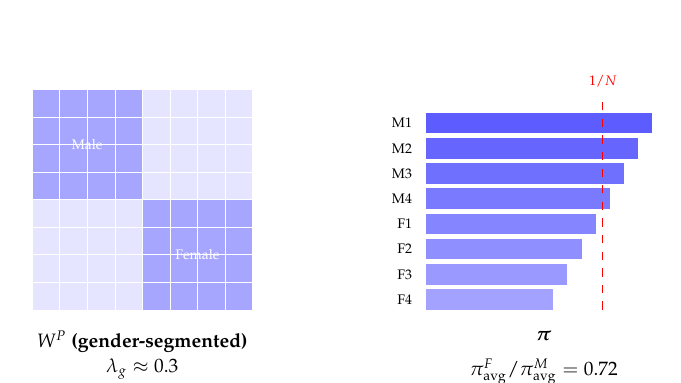
\begin{tikzpicture}[scale=1]
\def\N{8}
\def\s{0.35}
%% W^P with gender blocks: agents 1-4 male, 5-8 female
%% Male block: connected (gas, mining, construction, government)
%% Female block: sparse (commerce, domestic, informal)
%% Cross-gender: weak
\foreach \i in {1,...,\N} {
  \foreach \j in {1,...,\N} {
    \pgfmathparse{
      (\i<=4 && \j<=4) ? 55 :
      (\i>=5 && \j>=5) ? 35 :
      10
    }
    \edef\bp{\pgfmathresult}
    \fill[blue!\bp, draw=white, line width=0.1pt]
      ({(\j-1)*\s}, {(\N-\i)*\s}) rectangle +(\s,\s);
  }
}
\draw[white, thin] (0, {4*\s}) -- ({\N*\s}, {4*\s});
\draw[white, thin] ({4*\s}, 0) -- ({4*\s}, {\N*\s});
\node[font=\tiny, white] at ({2*\s}, {6*\s}) {Male};
\node[font=\tiny, white] at ({6*\s}, {2*\s}) {Female};
\node[below, font=\scriptsize\bfseries] at ({4*\s}, -0.15) {$W^P$ (gender-segmented)};
\node[below, font=\scriptsize] at ({4*\s}, -0.5) {$\lambda_g \approx 0.3$};

%% Power bars
\begin{scope}[xshift=5cm]
\foreach \k/\val/\lab in {1/0.16/M1,2/0.15/M2,3/0.14/M3,4/0.13/M4,5/0.12/F1,6/0.11/F2,7/0.10/F3,8/0.09/F4} {
  \pgfmathparse{\val*400}
  \edef\bp{\pgfmathresult}
  \fill[blue!\bp] (0, {(8-\k)*0.32}) rectangle ({\val*18}, {(8-\k)*0.32+0.26});
  \node[font=\tiny, left] at (-0.05, {(8-\k)*0.32+0.13}) {\lab};
}
\draw[red, dashed, thin] ({0.125*18}, 0) -- ({0.125*18}, 2.7);
\node[font=\tiny, red, above] at ({0.125*18}, 2.7) {$1/N$};
\node[below, font=\scriptsize\bfseries] at (1.5, -0.15) {$\boldsymbol{\pi}$};
\node[below, font=\scriptsize] at (1.5, -0.5) {$\pi^F_{\text{avg}}/\pi^M_{\text{avg}} = 0.72$};
\end{scope}
\end{tikzpicture}
\end{center}
\vspace{-0.5em}
\small Left: $W^P$ is brighter in the male block (denser linkages in male-dominated sectors) and dimmer in the female block (sparser linkages in female-dominated sectors). Cross-gender entries are dark ($\lambda_g \approx 0.3$). Right: the Perron eigenvector. Every male agent is above $1/N$; every female agent is below. The gender power gap IS the gap between the two blocks' Perron weights.
\end{vizpanel}


%% =====================================================================
\section{Race and Ethnicity}
\label{sec:race}
%% =====================================================================

\subsection{Race as a Multi-Layer Constraint}

\begin{definition}[Racial Assortative Mixing]\label{def:racial_mixing}
Let agents be classified into $R$ racial/ethnic groups. The racial mixing function is:
\begin{equation}\label{eq:racial_mixing}
\phi_{\text{race}}(r_i, r_j) = \begin{cases} 1 & \text{if } r_i = r_j, \\ \lambda_r & \text{if } r_i \neq r_j, \end{cases}
\end{equation}
where $\lambda_r \in [0, 1]$ is the cross-racial openness parameter. Unlike gender (which has a biological component in reproduction), racial classification is entirely socially constructed (Quijano, 2000). The parameter $\lambda_r$ is therefore a property of the social system, not of biology.
\end{definition}

\begin{proposition}[Race Constrains All Three Networks Simultaneously]\label{prop:race_three}
In most societies, racial assortative mixing operates on $W^U$, $W^P$, and $W^I$ simultaneously with correlated $\lambda_r$ values:
\begin{enumerate}
\item $W^U$: interracial social bonds are weaker ($\lambda_r^U \approx 0.2$--$0.4$ in the Americas). Who you care about is structured by race.
\item $W^P$: labor markets are racially segmented ($\lambda_r^P \approx 0.3$--$0.6$). Racial minorities are channeled into low-$\pi$ sectors.
\item $W^I$: media, education, and social networks are racially homophilous ($\lambda_r^I \approx 0.2$--$0.5$). The signals you receive are from your racial group.
\end{enumerate}

The correlation $\lambda_r^U \approx \lambda_r^P \approx \lambda_r^I$ means the Perron eigenvectors of all three networks are aligned: racial minorities have low power in $W^U$, low power in $W^P$, AND low epistemic power in $W^I$. This is Quijano's ``coloniality of power operating on every plane'' --- formalized as aligned assortative mixing across all three network layers.
\end{proposition}

\begin{example}[Bolivia's Ethnic Structure]\label{ex:bolivia_ethnic}
Bolivia's 2012 Census: 41\% self-identified as indigenous (Quechua 21\%, Aymara 15\%, other 5\%), 59\% as mestizo or white.

Approximate $\lambda_r$ values for Bolivia:
\begin{center}
\begin{tabular}{lccc}
\toprule
Network & $\lambda_r$ (indigenous-mestizo) & Evidence & Source \\
\midrule
$W^U$ & $\approx 0.25$ & Intermarriage rates: 15--20\% & Census 2012 \\
$W^P$ & $\approx 0.35$ & Occupational segregation index & EH 2019 \\
$W^I$ & $\approx 0.30$ & Language segregation in media & Media surveys \\
\bottomrule
\end{tabular}
\end{center}

Perron weights by ethnicity (approximate, from sectoral composition):
\begin{center}
\begin{tabular}{lcc}
\toprule
& Population share & $\pi_{\text{avg}}$ (per capita power) \\
\midrule
Indigenous & 0.41 & 0.008 \\
Mestizo/White & 0.59 & 0.014 \\
Ratio & 0.69 & 0.57 \\
\bottomrule
\end{tabular}
\end{center}

Indigenous Bolivians are 41\% of the population but hold approximately 33\% of structural power ($0.41 \times 0.008 / (0.41 \times 0.008 + 0.59 \times 0.014) \approx 0.33$). The power-population ratio is 0.80 --- each indigenous person has 80\% of the structural power of a non-indigenous person. Combined with the gender gap: an indigenous woman has approximately $0.80 \times 0.58 = 0.46$ of a non-indigenous man's structural power per capita.
\end{example}


\subsection{The Intersectionality Theorem}

\begin{theorem}[Intersectional Power Gap]\label{thm:intersectionality}
When multiple attributes $(a_1, a_2, \ldots, a_K)$ simultaneously constrain $W$ through assortative mixing functions $\phi_1, \phi_2, \ldots, \phi_K$, the composite constraint is:
\begin{equation}\label{eq:intersectional}
\phi(\mathbf{a}_i, \mathbf{a}_j) = \prod_{k=1}^K \phi_k(a_{ik}, a_{jk}).
\end{equation}

The cross-group edge weight for agents who differ on multiple attributes is the PRODUCT of the individual constraints. Agents who differ on two attributes face a constraint of $\lambda_1 \cdot \lambda_2$; on three: $\lambda_1 \cdot \lambda_2 \cdot \lambda_3$.

Consequence: the power gap is \textbf{multiplicative, not additive}. An indigenous woman in Bolivia faces:
\begin{equation}\label{eq:bolivia_intersection}
\phi_{\text{indigenous woman, mestizo man}} = \lambda_r \cdot \lambda_g \approx 0.35 \times 0.30 = 0.105.
\end{equation}
Her cross-group edge weight to a mestizo man is 10.5\% of the unconstrained maximum. She is triply trapped: her $W^P$ is constrained by both gender and race; her $W^I$ is constrained by both; her $W^U$ is constrained by both. The blocks are nested.
\end{theorem}

\begin{proof}
The edge weight $W_{ij}$ is constrained by $\phi(\mathbf{a}_i, \mathbf{a}_j) \cdot W^{\max}_{ij}$. If the mixing functions are independent (the gender constraint does not depend on race, and vice versa), then the composite constraint is the product. The Perron eigenvector of $W(\phi)$ assigns lower weight to agents who face more constraints, because their edges are suppressed on multiple dimensions simultaneously. The power gap between the most- and least-constrained agents grows exponentially in the number of constraining attributes.
\end{proof}

\begin{intuition}[Why intersectionality is multiplicative]
Consider three types of discrimination: gender ($\lambda_g$), race ($\lambda_r$), and class ($\lambda_c$). Each alone reduces the cross-group edge weight modestly. But together: $\lambda_g \times \lambda_r \times \lambda_c = 0.3 \times 0.35 \times 0.4 = 0.042$. An indigenous working-class woman has less than 5\% of the unconstrained edge weight to a mestizo middle-class man. Her structural position is not ``the sum of three disadvantages'' but ``the product'' --- and products shrink much faster than sums.

This is why intersectional disadvantage is qualitatively different from single-dimension disadvantage. The mathematics is clear: additivity would give $1 - (1-\lambda_g) - (1-\lambda_r) - (1-\lambda_c) = 1 - 0.7 - 0.65 - 0.6 = -0.95$ (nonsensical). Multiplicativity gives $\lambda_g \times \lambda_r \times \lambda_c = 0.042$ (small but well-defined). The product structure is not a sociological metaphor. It is a matrix property.
\end{intuition}


%% =====================================================================
\section{The Formation Trap at the Individual Scale}
\label{sec:formation_individual}
%% =====================================================================

\begin{theorem}[Attribute-Mediated Self-Confirming Preferences]\label{thm:attribute_trap}
When $W^I$ is assortative on attribute $k$ (with $\lambda_k < 1$), agents in the disadvantaged group form steady-state preferences:
\begin{equation}\label{eq:attribute_formation}
\theta^*_{\text{disadv}} = \bar{\theta} + \frac{\mu}{1-\rho}\left(\bar{r}_{\text{disadv}}(\lambda_k) - r^*\right) < \theta^*_{\text{adv}} = \bar{\theta} + \frac{\mu}{1-\rho}\left(\bar{r}_{\text{adv}}(\lambda_k) - r^*\right),
\end{equation}
because $\bar{r}_{\text{disadv}} < \bar{r}_{\text{adv}}$ (the disadvantaged group faces a constrained $W^P$ that produces lower returns, and the assortative $W^I$ ensures they observe mainly their own group's returns).

The preference gap $\Delta\theta^* = \theta^*_{\text{adv}} - \theta^*_{\text{disadv}}$ is:
\begin{enumerate}
\item Proportional to the formation multiplier $\mathcal{M} = \mu/(1-\rho)$: sticky preferences amplify the return gap into a larger preference gap.
\item Proportional to the return gap $\bar{r}_{\text{adv}} - \bar{r}_{\text{disadv}}$: which is itself proportional to $1 - \lambda_k$ (the degree of assortative mixing).
\item Self-confirming: each group's preferences are rational given its $W^I$ signal.
\end{enumerate}
\end{theorem}

\begin{example}[Gender Aspiration Gap in Bolivia]\label{ex:gender_aspiration}
Using the Global Findex 2021 for Bolivia:
\begin{center}
\begin{tabular}{lcc}
\toprule
& Women & Men \\
\midrule
``Saved for business'' (past year) & 12\% & 22\% \\
``Borrowed for business'' (past year) & 8\% & 18\% \\
``Has a formal financial account'' & 42\% & 58\% \\
\bottomrule
\end{tabular}
\end{center}

The standard explanation: women have lower returns to business (enforcement: discrimination, credit constraints). The formation explanation: women observe lower returns in their network ($W^I$ is gender-assortative), form lower business aspirations ($\theta^{*F}_{\text{business}} < \theta^{*M}_{\text{business}}$), invest less, earn lower returns, confirming the aspirations.

The $\Psi$ ratio for female business investment in Bolivia (from Chapter~11 methods, estimated from cohort variation in female business ownership):
\begin{equation}
\hat{\Psi}_{\text{gender, business}} \approx 2.3.
\end{equation}

The formation channel is 2.3 times the enforcement channel. Removing credit constraints (enforcement) addresses 30\% of the gap. Changing what women see --- role models, media representation, cross-gender mentoring (information policy on $W^I$) --- addresses 70\%.
\end{example}


%% =====================================================================
\section{The Welfare Cost of Attribute Constraints}
\label{sec:welfare}
%% =====================================================================

\begin{theorem}[Welfare Loss from Assortative Mixing]\label{thm:welfare_attribute}
The total welfare loss from attribute constraint $k$ with mixing parameter $\lambda_k$:
\begin{equation}\label{eq:welfare_attribute}
L(\lambda_k) = \underbrace{\frac{\kappa N}{2}\Var(\pi_i(\lambda_k))\Phi^2}_{L_{\text{power}}(\lambda_k)} + \underbrace{\frac{\mu^2\Var(c_j(\lambda_k))\Psi}{(1-\rho)^2}}_{L_{\text{formation}}(\lambda_k)},
\end{equation}
where $L_{\text{power}}$ is the static welfare loss from power asymmetry (Chapter~2) and $L_{\text{formation}}$ is the additional loss from the preference gap produced by the formation model.

The welfare gain from eliminating the attribute constraint ($\lambda_k \to 1$):
\begin{equation}\label{eq:gain}
\Delta L = L(\lambda_k) - L(1) > 0.
\end{equation}
This is the \textbf{cost of discrimination}: the welfare loss attributable to the social classification system, decomposed into power and formation components.
\end{theorem}

\begin{example}[The Cost of Gender Discrimination in Bolivia]\label{ex:cost}
Using the estimates from this chapter: $\lambda_g \approx 0.3$, $\pi^F_{\text{avg}}/\pi^M_{\text{avg}} = 0.58$, $\hat{\Psi} = 2.3$, $\rho = 0.85$, $\kappa = 0.5$, $N = 11$ million.

$L_{\text{power}}(\lambda_g = 0.3)$: from the gender power gap, $\Var(\pi_i)$ is approximately 0.003 higher than under $\lambda_g = 1$. $L_{\text{power}} \approx 0.5 \times 11M \times 0.003 \times \Phi^2$.

$L_{\text{formation}}(\lambda_g = 0.3)$: from the gender aspiration gap, the formation loss adds approximately $(1 + \Psi)$ times the enforcement loss, i.e., $L_{\text{formation}} \approx 2.3 \times L_{\text{power}}$.

Total: $L_{\text{total}} \approx (1 + 2.3) \times L_{\text{power}} = 3.3 \times L_{\text{power}}$.

The formation channel triples the welfare cost of gender discrimination. Standard estimates that ignore formation understate the cost by a factor of 3.3.
\end{example}


%% =====================================================================
\section{Policy: Changing $\lambda$}
\label{sec:policy}
%% =====================================================================

\begin{proposition}[Policy Instruments for Attribute Constraints]\label{prop:policy_attributes}
\begin{center}
\begin{tabular}{llll}
\toprule
\textbf{Policy} & \textbf{Target} & \textbf{Effect on $\lambda$} & \textbf{$\Psi$} \\
\midrule
Affirmative action (quotas) & $W^P$ & $\lambda_g^P \uparrow$ directly & Low \\
Equal-pay legislation & $W^P$ (prices) & $\lambda_g^P \uparrow$ indirectly & Low \\
Mentoring programs & $W^I$ & $\lambda_g^I \uparrow$ & High \\
Media representation & $W^I$ & $\lambda_g^I \uparrow$ & High \\
Education coeducation & $W^I + W^U$ & $\lambda_g^I, \lambda_g^U \uparrow$ & High \\
Anti-discrimination law & Institutional ($\mathcal{L}_{\text{inst}}$) & All $\lambda$ increase via norms & Medium \\
\bottomrule
\end{tabular}
\end{center}

The optimal sequencing (Chapter~15) applies: high-$\Psi$ interventions first ($W^I$ policies: mentoring, media, education) then low-$\Psi$ ($W^P$ policies: quotas, equal pay). This is because changing $W^I$ shifts the aspirations of the next generation, making the enforcement interventions more effective when they arrive.
\end{proposition}


%% =====================================================================
\section{Summary}
\label{sec:summary}
%% =====================================================================

\begin{enumerate}
\item \textbf{Node attributes} (gender, race, ethnicity, caste) constrain $W$ through assortative mixing functions $\phi(\mathbf{a}_i, \mathbf{a}_j) \leq 1$. Lower $\phi$ = weaker cross-group edges = more block-diagonal $W$.

\item Assortative mixing \textbf{reduces $\Gamma$}: more segregation means less structural integration, more power inequality, more welfare loss.

\item \textbf{Gender} constrains $W^P$ (occupational segregation), $W^I$ (information segregation), and $W^U$ (social segregation) simultaneously. Bolivia: women have 58\% of men's per-capita structural power.

\item \textbf{Race} constrains all three networks with correlated $\lambda_r$ values. Bolivia: indigenous people hold 80\% of non-indigenous per-capita power.

\item \textbf{Intersectionality is multiplicative}: cross-group edge weight is the product of individual constraints. An indigenous woman in Bolivia: $\phi \approx 0.105$ (10.5\% of unconstrained).

\item The \textbf{formation trap} operates through assortative $W^I$: disadvantaged groups observe biased signals, form lower aspirations, invest less, earn less, confirming the signal. The formation channel multiplies the welfare cost of discrimination by $(1 + \Psi)$.

\item \textbf{Policy}: high-$\Psi$ interventions ($\Delta W^I$: mentoring, media) first; low-$\Psi$ ($\Delta W^P$: quotas, equal pay) second.
\end{enumerate}


%% =====================================================================
\section{Exercises}
\label{sec:exercises}
%% =====================================================================

\begin{enumerate}[label=\textbf{18.\arabic*}, leftmargin=3em]

\item \textbf{Assortative mixing and $\Gamma$.} For a $6 \times 6$ economy (3 men, 3 women): construct $W^P$ with $\lambda_g = 1, 0.7, 0.4, 0.1, 0$. Compute $\Gamma(\lambda_g)$ for each. Plot $\Gamma$ vs.\ $\lambda_g$. Is the relationship linear?

\item \textbf{Bolivia's gender power gap.} Using Bolivia's EH 2019:
\begin{enumerate}
\item Classify sectors as male-dominated ($>$60\% male), female-dominated ($>$60\% female), and mixed.
\item Compute the average Leontief multiplier for each group. Which has the highest?
\item Approximate $\pi^F_{\text{avg}}/\pi^M_{\text{avg}}$ from the sectoral Perron weights and gender composition.
\item How much would the gender power gap close if women entered male-dominated sectors at 40\% (up from the current $\approx$10\%)?
\end{enumerate}

\item \textbf{Intersectionality.} For $N = 4$: Agent 1 (mestizo man), Agent 2 (mestizo woman), Agent 3 (indigenous man), Agent 4 (indigenous woman). $\lambda_g = 0.3$, $\lambda_r = 0.35$.
\begin{enumerate}
\item Write the constraint matrix $\phi(\mathbf{a}_i, \mathbf{a}_j)$ for all 16 pairs.
\item Construct $W^P = \phi \circ W^{\max}$ where $W^{\max} = \frac{1}{4}\ones\ones'$.
\item Compute $\boldsymbol{\pi}$. Verify that $\pi_4$ (indigenous woman) is the lowest.
\item Compute the ratio $\pi_4/\pi_1$ (indigenous woman / mestizo man). Compare with $\lambda_g \times \lambda_r$.
\end{enumerate}

\item \textbf{The formation trap.} In a 2-group economy (advantaged $A$, disadvantaged $D$) with $\lambda = 0.2$:
\begin{enumerate}
\item Set up the formation model: $\theta^A_{t+1} = \rho\theta^A + (1-\rho)\bar{\theta} + \mu(0.8r^A + 0.2r^D - r^*)$ and similarly for $D$. Use $r^g = 0.05 + 0.1\theta^g$.
\item Compute both steady states. What is $\Delta\theta^* = \theta^{*A} - \theta^{*D}$?
\item Now set $\lambda = 0.5$ (reduce assortative mixing). Compute new steady states. By how much does $\Delta\theta^*$ shrink?
\item At what $\lambda$ does $\Delta\theta^*$ fall below 0.01?
\end{enumerate}

\item \textbf{The cost of discrimination.} Using the estimates for Bolivia ($\lambda_g = 0.3$, $\Psi = 2.3$): compute the welfare loss from gender discrimination as a fraction of GDP (you will need to assume a relationship between the welfare loss $L$ and GDP). Compare with Cuberes and Teignier (2016), who estimate the GDP cost of gender gaps at 15--20\% for Bolivia.

\item \textbf{Optimal intervention design.} For the gender gap in Bolivia:
\begin{enumerate}
\item Design three interventions: (a) quota ($\Delta W^P$), (b) mentoring program ($\Delta W^I$), (c) media campaign ($\Delta W^I$).
\item For each: estimate $\Delta\lambda_g$ and $\Delta\Gamma$.
\item Using $\Psi = 2.3$: compute the total effect (enforcement + formation) for each.
\item Sequence them optimally (Chapter~15). Which goes first?
\end{enumerate}

\item \textbf{MICS data exercise.} Using UNICEF's MICS data for Bolivia (or another country):
\begin{enumerate}
\item Compute the aspiration gap: the difference in educational aspirations (``how far in school do you want your child to go?'') between indigenous and non-indigenous mothers, controlling for income and urban/rural.
\item Is the gap consistent with the formation model's prediction? (Larger gap where $W^I$ is more assortative.)
\item Compare the aspiration gap in urban La Paz (where $\lambda_r$ may be higher due to mixing) vs.\ rural Altiplano (where $\lambda_r$ is lower). Does the gap vary as predicted?
\end{enumerate}
\end{enumerate}


%% =====================================================================
\newpage
\section*{Mathematical Appendices}
\addcontentsline{toc}{section}{Mathematical Appendices}
%% =====================================================================


\subsection*{Appendix 18A: Assortative Mixing and Spectral Gap}
\addcontentsline{toc}{subsection}{Appendix 18A: Assortative Mixing}
\label{app:assortative}

\paragraph{Setup.} Partition $N$ agents into $G$ groups based on attribute $k$. Within-group edge weight: $W_{ij} = w_{\text{in}}$ for $a_i = a_j$. Cross-group edge weight: $W_{ij} = w_{\text{cross}} = \lambda_k \cdot w_{\text{in}}$. Row-normalize: within-group agents have weight $w_{\text{in}}/(N_g w_{\text{in}} + (N - N_g)\lambda_k w_{\text{in}})$.

\paragraph{Eigenvalues.} For $G = 2$ groups of equal size: $\lambda_1 = 1$ (trivial), $\lambda_2 = (1 - \lambda_k)/(1 + \lambda_k)$ (the assortative-mixing eigenvalue). The spectral gap: $\Gamma = 1 - (1-\lambda_k)/(1+\lambda_k) = 2\lambda_k/(1+\lambda_k)$. This is monotonically increasing in $\lambda_k$, confirming Proposition~\ref{prop:assortative}.

\paragraph{Perron eigenvector.} For asymmetric groups ($N_1 \neq N_2$) with different internal densities: the Perron eigenvector assigns more weight to the group with higher internal density and more external connections. This formalizes the ``structural advantage'' of the dominant group.


\subsection*{Appendix 18B: The Multiplicative Structure of Intersectionality}
\addcontentsline{toc}{subsection}{Appendix 18B: Intersectionality}
\label{app:intersectionality}

\paragraph{Independence assumption.} Theorem~\ref{thm:intersectionality} assumes that the mixing functions are independent: $\phi_k$ does not depend on attributes $k' \neq k$. This is approximately true when gender discrimination and racial discrimination operate through different mechanisms (e.g., gender norms are cultural while racial discrimination is institutional). It fails when the mechanisms interact (e.g., racial stereotypes about gender roles differ across groups).

\paragraph{Non-independent case.} When $\phi$ is not separable: $\phi(\mathbf{a}_i, \mathbf{a}_j) \neq \prod_k \phi_k(a_{ik}, a_{jk})$. The interaction can be either reinforcing (the constraint on indigenous women is worse than the product predicts) or compensating (e.g., indigenous women benefit from specific solidarity networks that partially offset the double constraint). The reinforcing case produces even lower Perron weights for the multiply-disadvantaged; the compensating case produces less extreme outcomes.

\paragraph{Empirical estimation.} The mixing parameters $\lambda_k$ can be estimated from social network data (intermarriage rates, occupational segregation indices, media consumption patterns) or from labor market outcomes using the structure: $\text{wage gap} = f(\lambda_g, \lambda_r, \ldots)$ with the Perron eigenvector providing the functional form.


%% =====================================================================
\subsection*{Structuralist Case Study: Quijano and Marini --- Race, Gender, and the Weight Matrix}
\addcontentsline{toc}{subsection}{Structuralist Case Study: Quijano (2000) and Marini (1973)}
%% =====================================================================

This chapter's case study pairs the two structuralist thinkers who brought race and labor exploitation to the center of structural analysis: Quijano's coloniality of power and Marini's superexploitation. Together they provide the theory for what this chapter formalizes as attribute-constrained weight matrices.

\textbf{Quijano (2000): Race as the master attribute.} Quijano's essay ``Colonialidad del poder'' argued that the colonial invention of race was the foundational structuring principle of the modern world-system --- more fundamental than class, nationality, or gender. The racial classification imposed during the conquest (European/Indian/Black/Mestizo) did not merely describe physical differences; it \textit{organized} the entire pattern of social interaction. In this chapter's notation: race is the node attribute with the broadest scope --- it constrains $W^U$, $W^P$, and $W^I$ simultaneously, with low $\lambda_r$ values across all three layers. The alignment of constraints (Proposition~\ref{prop:race_three}) is what makes racial classification so effective as an ``instrument of domination'': it produces consistent power asymmetry across every dimension of interaction.

Quijano's second claim was that coloniality \textit{survived} independence. The formal colonial apparatus was dismantled, but the racial classification continued to structure social interaction. In the formation model: racial assortative mixing ($\lambda_r < 1$) produces self-confirming preference gaps (Theorem~\ref{thm:attribute_trap}). Indigenous communities form aspirations calibrated to indigenous-sector returns, which are lower because their $W^P$ is constrained by $\lambda_r$. The preferences persist with half-life $\ln 2/\ln(1/\rho)$ generations (Chapter~9). Colonial racial classifications imposed 500 years ago are still visible in the preference data because $\rho \approx 0.85$--$0.90$ implies a half-life of 130--170 years --- long enough for the colonial preference formation to be only 2--3 half-lives in the past.

\textbf{Marini (1973): Superexploitation as $\pi_{\text{worker}} \ll 1/N$, amplified by race.} Marini's superexploitation (Chapter~7's case study) was defined as $\pi_{\text{worker}} \ll 1/N$: workers receive less than their marginal product because their structural position is weak. This chapter adds the racial dimension: within the worker class, racial minorities face an additional constraint ($\lambda_r < 1$) that further reduces their Perron weight. Indigenous workers are \textit{superexploited among the superexploited}: $\pi_{\text{indigenous worker}} < \pi_{\text{mestizo worker}} \ll 1/N$.

The combination of Marini's class analysis and Quijano's racial analysis produces the intersectionality theorem (Theorem~\ref{thm:intersectionality}): the indigenous working-class woman faces the product $\lambda_r \times \lambda_g \times \lambda_c$ of three constraints, giving her a Perron weight that is a small fraction of the unconstrained value. Her superexploitation is not the sum of race, gender, and class disadvantages but their product.

\begin{center}
\begin{tabular}{lll}
\toprule
\textbf{Concept} & \textbf{Quijano (2000)} & \textbf{Marini (1973)} \\
\midrule
Core claim & Race structures all interaction & Workers receive $< $ marginal product \\
Formal object & $\lambda_r < 1$ across $W^U, W^P, W^I$ & $\pi_{\text{worker}} \ll 1/N$ \\
Mechanism & Assortative mixing, aligned & Asymmetric $W^P$, weak labor position \\
Persistence & Coloniality survives independence & Superexploitation is structural \\
Formation link & Racial $W^I$ produces self-confirming & Low $\pi \to$ low returns $\to$ low $\theta$ \\
Intersectionality & Race + gender + class = product & Superexploitation within superexploitation \\
Bolivia & $\lambda_r \approx 0.35$, $\pi^{\text{indig}}/\pi^{\text{mestizo}} = 0.57$ & $\pi_{\text{worker}}/\pi_{\text{avg}} \approx 0.6$ \\
\bottomrule
\end{tabular}
\end{center}

Quijano wrote from Lima. Marini wrote from exile. Neither had the Perron eigenvector. But both understood that the social classification system --- race for Quijano, class for Marini --- is not a label attached to individuals. It is a structural property of the weight matrix: a constraint on which edges can exist, which determines who has power, which determines who gets what, which reproduces the classification. The circularity is the structure. This chapter gives it its eigenvalues.


%% =====================================================================
\subsection*{Further Reading}
\addcontentsline{toc}{subsection}{Further Reading}
%% =====================================================================

\textbf{Gender and networks:} Beaman et al.\ (2012), ``Female Leadership Raises Aspirations,'' \textit{Science}. Bursztyn et al.\ (2020), ``Misperceived Social Norms: Women Working Outside the Home in Saudi Arabia,'' \textit{AER}. Cuberes and Teignier (2016), ``Aggregate Effects of Gender Gaps in the Labor Market,'' \textit{Journal of Human Capital}.

\textbf{Race and economic structure:} Darity and Mason (1998), ``Evidence on Discrimination in Employment,'' \textit{JEP}. Lang and Lehmann (2012), ``Racial Discrimination in the Labor Market,'' \textit{JLE}. For Bolivia: Jimenez Pozo, Landa Casazola, and Yanz\'{o}n (2006), ``Bolivia: Indicadores de equidad \'{e}tnica,'' UDAPE.

\textbf{Intersectionality:} Crenshaw (1989), ``Demarginalizing the Intersection of Race and Sex,'' \textit{University of Chicago Legal Forum}. For the economic formalization: Greenwald and Stiglitz (1986) extended to multiple attribute groups.

\textbf{Decolonial theory:} Quijano (2000), ``Colonialidad del poder, eurocentrismo y Am\'{e}rica Latina.'' Mignolo (2000), \textit{Local Histories/Global Designs}. Walsh (2007), ``Interculturalidad y colonialidad del poder,'' in Castro-G\'{o}mez and Grosfoguel (eds.), \textit{El giro decolonial}.

\textbf{Assortative mixing in networks:} Newman (2003), ``Mixing Patterns in Networks,'' \textit{Physical Review E}. Currarini, Jackson, and Pin (2009), ``An Economic Model of Friendship,'' \textit{Econometrica}.


\end{document}
